%%%%%%%%%%%%%%%%%%%%%%%%%%%%%%%%%%%%%%%%%
%  My documentation report
%  Objetive: Explain what I did and how, so someone can continue with the investigation
%
% Important note:
% Chapter heading images should have a 2:1 width:height ratio,
% e.g. 920px width and 460px height.
%
%%%%%%%%%%%%%%%%%%%%%%%%%%%%%%%%%%%%%%%%%


%----------------------------------------------------------------------------------------
%	PACKAGES AND OTHER DOCUMENT CONFIGURATIONS
%----------------------------------------------------------------------------------------

\documentclass[fleqn]{book} % Default font size and left-justified equations
%\documentclass[1pt]{article} % Imposta tutto il testo base a 12 punti
\usepackage[top=3cm,bottom=3cm,left=3.2cm,right=3.2cm,headsep=10pt,letterpaper]{geometry} % Page margins

\usepackage{xcolor} % Required for specifying colors by name
\definecolor{ocre}{RGB}{52,177,201} % Define the orange color used for highlighting throughout the book

% Font Settings
\usepackage{avant} % Use the Avantgarde font for headings
%\usepackage{times} % Use the Times font for headings
\usepackage{mathptmx} % Use the Adobe Times Roman as the default text font together with math symbols from the Sym­bol, Chancery and Com­puter Modern fonts
\usepackage{microtype} % Slightly tweak font spacing for aesthetics
\usepackage[utf8]{inputenc} % Required for including letters with accents
\usepackage[T1]{fontenc} % Use 8-bit encoding that has 256 glyphs
\usepackage{amsthm}

% Bibliography
\usepackage{csquotes} % Required for biblatex
\usepackage[backend=biber, style=numeric]{biblatex}
\addbibresource{bibliography.bib} % BibTeX bibliography file
\defbibheading{bibempty}{}
\DeclareUnicodeCharacter{2060}{\hspace{0pt}}

%----------------------------------------------------------------------------------------
%	VARIOUS REQUIRED PACKAGES
%----------------------------------------------------------------------------------------

\usepackage{titlesec} % Allows customization of titles
\usepackage{setspace} % Allows for setting the spacing between lines

\usepackage{graphicx} % Required for including pictures
\graphicspath{{Pictures/}} % Specifies the directory where pictures are stored
% \graphicspath{{Plots/}}
\usepackage{lipsum} % Inserts dummy text

\usepackage{tikz} % Required for drawing custom shapes

\usepackage[english]{babel} % English language/hyphenation

\usepackage{enumitem} % Customize lists
\setlist{nolistsep} % Reduce spacing between bullet points and numbered lists

\usepackage{booktabs} % Required for nicer horizontal rules in tables

\usepackage{eso-pic} % Required for specifying an image background in the title page

%----------------------------------------------------------------------------------------
%	MAIN TABLE OF CONTENTS
%----------------------------------------------------------------------------------------

\usepackage{titletoc} % Required for manipulating the table of contents

\contentsmargin{0cm} % Removes the default margin
% Chapter text styling
\titlecontents{chapter}[1.25cm] % Indentation
{\addvspace{15pt}\large\sffamily\bfseries} % Spacing and font options for chapters
{\color{ocre!60}\contentslabel[\Large\thecontentslabel]{1.25cm}\color{ocre}} % Chapter number
{}  
{\color{ocre!60}\normalsize\sffamily\bfseries\;\titlerule*[.5pc]{.}\;\thecontentspage} % Page number
% Section text styling
\titlecontents{section}[1.25cm] % Indentation
{\addvspace{5pt}\sffamily\bfseries} % Spacing and font options for sections
{\contentslabel[\thecontentslabel]{1.25cm}} % Section number
{}
{\sffamily\hfill\color{black}\thecontentspage} % Page number
[]
% Subsection text styling
\titlecontents{subsection}[1.25cm] % Indentation
{\addvspace{1pt}\sffamily\small} % Spacing and font options for subsections
{\contentslabel[\thecontentslabel]{1.25cm}} % Subsection number
{}
{\sffamily\;\titlerule*[.5pc]{.}\;\thecontentspage} % Page number
[] 

%----------------------------------------------------------------------------------------
%	MINI TABLE OF CONTENTS IN CHAPTER HEADS
%----------------------------------------------------------------------------------------

% Section text styling
\titlecontents{lsection}[0em] % Indendating
{\footnotesize\sffamily} % Font settings
{}
{}
{}

% Subsection text styling
\titlecontents{lsubsection}[.5em] % Indentation
{\normalfont\footnotesize\sffamily} % Font settings
{}
{}
{}
 
%----------------------------------------------------------------------------------------
%	PAGE HEADERS
%----------------------------------------------------------------------------------------

\usepackage{fancyhdr} % Required for header and footer configuration

\pagestyle{fancy}
\renewcommand{\chaptermark}[1]{\markboth{\sffamily\normalsize\bfseries\chaptername\ \thechapter.\ #1}{}} % Chapter text font settings
\renewcommand{\sectionmark}[1]{\markright{\sffamily\normalsize\thesection\hspace{5pt}#1}{}} % Section text font settings
\fancyhf{} \fancyhead[LE,RO]{\sffamily\normalsize\thepage} % Font setting for the page number in the header
\fancyhead[LO]{\rightmark} % Print the nearest section name on the left side of odd pages
\fancyhead[RE]{\leftmark} % Print the current chapter name on the right side of even pages
\renewcommand{\headrulewidth}{0.5pt} % Width of the rule under the header
\addtolength{\headheight}{2.5pt} % Increase the spacing around the header slightly
\renewcommand{\footrulewidth}{0pt} % Removes the rule in the footer
\fancypagestyle{plain}{\fancyhead{}\renewcommand{\headrulewidth}{0pt}} % Style for when a plain pagestyle is specified

% Removes the header from odd empty pages at the end of chapters
\makeatletter
\renewcommand{\cleardoublepage}{
\clearpage\ifodd\c@page\else
\hbox{}
\vspace*{\fill}
\thispagestyle{empty}
\newpage
\fi}

%----------------------------------------------------------------------------------------
%	THEOREM STYLES
%----------------------------------------------------------------------------------------

\usepackage{amsmath,amsfonts,amssymb,amsthm} % For math equations, theorems, symbols, etc

\newcommand{\intoo}[2]{\mathopen{]}#1\,;#2\mathclose{[}}
\newcommand{\ud}{\mathop{\mathrm{{}d}}\mathopen{}}
\newcommand{\intff}[2]{\mathopen{[}#1\,;#2\mathclose{]}}
\newtheorem{notation}{Notation}[chapter]

%%%%%%%%%%%%%%%%%%%%%%%%%%%%%%%%%%%%%%%%%%%%%%%%%%%%%%%%%%%%%%%%%%%%%%%%%%%
%%%%%%%%%%%%%%%%%%%% dedicated to boxed/framed environements %%%%%%%%%%%%%%
%%%%%%%%%%%%%%%%%%%%%%%%%%%%%%%%%%%%%%%%%%%%%%%%%%%%%%%%%%%%%%%%%%%%%%%%%%%
\newtheoremstyle{ocrenumbox}% % Theorem style name
{0pt}% Space above
{0pt}% Space below
{\normalfont}% % Body font
{}% Indent amount
{\small\bf\sffamily\color{ocre}}% % Theorem head font
{\;}% Punctuation after theorem head
{0.25em}% Space after theorem head
{\small\sffamily\color{ocre}\thmname{#1}\nobreakspace\thmnumber{\@ifnotempty{#1}{}\@upn{#2}}% Theorem text (e.g. Theorem 2.1)
\thmnote{\nobreakspace\the\thm@notefont\sffamily\bfseries\color{black}---\nobreakspace#3.}} % Optional theorem note
\renewcommand{\qedsymbol}{$\blacksquare$}% Optional qed square

\newtheoremstyle{blacknumex}% Theorem style name
{5pt}% Space above
{5pt}% Space below
{\normalfont}% Body font
{} % Indent amount
{\small\bf\sffamily}% Theorem head font
{\;}% Punctuation after theorem head
{0.25em}% Space after theorem head
{\small\sffamily{\tiny\ensuremath{\blacksquare}}\nobreakspace\thmname{#1}\nobreakspace\thmnumber{\@ifnotempty{#1}{}\@upn{#2}}% Theorem text (e.g. Theorem 2.1)
\thmnote{\nobreakspace\the\thm@notefont\sffamily\bfseries---\nobreakspace#3.}}% Optional theorem note

\newtheoremstyle{blacknumbox} % Theorem style name
{0pt}% Space above
{0pt}% Space below
{\normalfont}% Body font
{}% Indent amount
{\small\bf\sffamily}% Theorem head font
{\;}% Punctuation after theorem head
{0.25em}% Space after theorem head
{\small\sffamily\thmname{#1}\nobreakspace\thmnumber{\@ifnotempty{#1}{}\@upn{#2}}% Theorem text (e.g. Theorem 2.1)
\thmnote{\nobreakspace\the\thm@notefont\sffamily\bfseries---\nobreakspace#3.}}% Optional theorem note

%%%%%%%%%%%%%%%%%%%%%%%%%%%%%%%%%%%%%%%%%%%%%%%%%%%%%%%%%%%%%%%%%%%%%%%%%%%
%%%%%%%%%%%%% dedicated to non-boxed/non-framed environements %%%%%%%%%%%%%
%%%%%%%%%%%%%%%%%%%%%%%%%%%%%%%%%%%%%%%%%%%%%%%%%%%%%%%%%%%%%%%%%%%%%%%%%%%
\newtheoremstyle{ocrenum}% % Theorem style name
{5pt}% Space above
{5pt}% Space below
{\normalfont}% % Body font
{}% Indent amount
{\small\bf\sffamily\color{ocre}}% % Theorem head font
{\;}% Punctuation after theorem head
{0.25em}% Space after theorem head
{\small\sffamily\color{ocre}\thmname{#1}\nobreakspace\thmnumber{\@ifnotempty{#1}{}\@upn{#2}}% Theorem text (e.g. Theorem 2.1)
\thmnote{\nobreakspace\the\thm@notefont\sffamily\bfseries\color{black}---\nobreakspace#3.}} % Optional theorem note
\renewcommand{\qedsymbol}{$\blacksquare$}% Optional qed square
\makeatother

% Defines the theorem text style for each type of theorem to one of the three styles above
\newcounter{dummy} 
\numberwithin{dummy}{section}
\theoremstyle{ocrenumbox}


\newtheorem{theoremeT}[dummy]{Theorem}
\newtheorem{lemma}[dummy]{Lemma}
\newtheorem{observation}[dummy]{Observation}
\newtheorem{proposition}[dummy]{Proposition}
% \newtheorem{definition}[dummy]{Definition}
\newtheorem{claim}[dummy]{Claim}
\newtheorem{fact}[dummy]{Fact}
\newtheorem{assumption}[dummy]{Assumption}

\newtheorem{problem}{Problem}[chapter]
% \newtheorem{exercise}{Exercise}[chapter]
\theoremstyle{blacknumex}
\newtheorem{exampleT}{Example}[chapter]
\theoremstyle{blacknumbox}
\newtheorem{vocabulary}{Vocabulary}[chapter]
\newtheorem{definitionT}{Definition}[section]
\newtheorem{corollaryT}[dummy]{Corollary}
\theoremstyle{ocrenum}

%----------------------------------------------------------------------------------------
%	DEFINITION OF COLORED BOXES
%----------------------------------------------------------------------------------------

\RequirePackage[framemethod=default]{mdframed} % Required for creating the theorem, definition, exercise and corollary boxes

% Theorem box
\newmdenv[skipabove=7pt,
skipbelow=7pt,
backgroundcolor=black!5,
linecolor=ocre,
innerleftmargin=5pt,
innerrightmargin=5pt,
innertopmargin=5pt,
leftmargin=0cm,
rightmargin=0cm,
innerbottommargin=5pt]{tBox}

% Exercise box	  
\newmdenv[skipabove=7pt,
skipbelow=7pt,
rightline=false,
leftline=true,
topline=false,
bottomline=false,
backgroundcolor=ocre!10,
linecolor=ocre,
innerleftmargin=5pt,
innerrightmargin=5pt,
innertopmargin=5pt,
innerbottommargin=5pt,
leftmargin=0cm,
rightmargin=0cm,
linewidth=4pt]{eBox}	

% Definition box
\newmdenv[skipabove=7pt,
skipbelow=7pt,
rightline=false,
leftline=true,
topline=false,
bottomline=false,
linecolor=ocre,
innerleftmargin=5pt,
innerrightmargin=5pt,
innertopmargin=0pt,
leftmargin=0cm,
rightmargin=0cm,
linewidth=4pt,
innerbottommargin=0pt]{dBox}	

% Corollary box
\newmdenv[skipabove=7pt,
skipbelow=7pt,
rightline=false,
leftline=true,
topline=false,
bottomline=false,
linecolor=gray,
backgroundcolor=black!5,
innerleftmargin=5pt,
innerrightmargin=5pt,
innertopmargin=5pt,
leftmargin=0cm,
rightmargin=0cm,
linewidth=4pt,
innerbottommargin=5pt]{cBox}

% Creates an environment for each type of theorem and assigns it a theorem text style from the "Theorem Styles" section above and a colored box from above
\newenvironment{theorem}{\begin{tBox}\begin{theoremeT}}{\end{theoremeT}\end{tBox}}
\newenvironment{exercise}{\begin{eBox}\begin{exerciseT}}{\hfill{\color{ocre}\tiny\ensuremath{\blacksquare}}\end{exerciseT}\end{eBox}}				  
\newenvironment{definition}{\begin{dBox}\begin{definitionT}}{\end{definitionT}\end{dBox}}	
\newenvironment{example}{\begin{exampleT}}{\hfill{\tiny\ensuremath{\blacksquare}}\end{exampleT}}		
\newenvironment{corollary}{\begin{cBox}\begin{corollaryT}}{\end{corollaryT}\end{cBox}}	

%----------------------------------------------------------------------------------------
%	REMARK ENVIRONMENT
%----------------------------------------------------------------------------------------

\newenvironment{remark}{\par\vspace{10pt}\small % Vertical white space above the remark and smaller font size
\begin{list}{}{
\leftmargin=35pt % Indentation on the left
\rightmargin=25pt}\item\ignorespaces % Indentation on the right
\makebox[-2.5pt]{\begin{tikzpicture}[overlay]
\node[draw=ocre!60,line width=1pt,circle,fill=ocre!25,font=\sffamily\bfseries,inner sep=2pt,outer sep=0pt] at (-15pt,0pt){\textcolor{ocre}{R}};\end{tikzpicture}} % Orange R in a circle
\advance\baselineskip -1pt}{\end{list}\vskip5pt} % Tighter line spacing and white space after remark

%----------------------------------------------------------------------------------------
%	SECTION NUMBERING IN THE MARGIN
%----------------------------------------------------------------------------------------

\makeatletter
\renewcommand{\@seccntformat}[1]{\llap{\textcolor{ocre}{\csname the#1\endcsname}\hspace{1em}}}                    
\renewcommand{\section}{\@startsection{section}{1}{\z@}
{-4ex \@plus -1ex \@minus -.4ex}
{1ex \@plus.2ex }
{\normalfont\large\sffamily\bfseries}}
\renewcommand{\subsection}{\@startsection {subsection}{2}{\z@}
{-3ex \@plus -0.1ex \@minus -.4ex}
{0.5ex \@plus.2ex }
{\normalfont\sffamily\bfseries}}
\renewcommand{\subsubsection}{\@startsection {subsubsection}{3}{\z@}
{-2ex \@plus -0.1ex \@minus -.2ex}
{.2ex \@plus.2ex }
{\normalfont\small\sffamily\bfseries}}                        
\renewcommand\paragraph{\@startsection{paragraph}{4}{\z@}
{-2ex \@plus-.2ex \@minus .2ex}
{.1ex}
{\normalfont\small\sffamily\bfseries}}

%----------------------------------------------------------------------------------------
%	HYPERLINKS IN THE DOCUMENTS
%----------------------------------------------------------------------------------------

% For an unclear reason, the package should be loaded now and not later
\usepackage{hyperref}
\hypersetup{hidelinks,colorlinks=false,breaklinks=true,urlcolor=ocre,bookmarksopen=false,pdftitle={Advanced Machine Learning},pdfauthor={Vincenzo Salvatore}}

%----------------------------------------------------------------------------------------
%	CHAPTER HEADINGS
%----------------------------------------------------------------------------------------

% The set-up below should be (sadly) manually adapted to the overall margin page septup controlled by the geometry package loaded in the main.tex document. It is possible to implement below the dimensions used in the goemetry package (top,bottom,left,right)... TO BE DONE

\newcommand{\thechapterimage}{}
\newcommand{\chapterimage}[1]{\renewcommand{\thechapterimage}{#1}}

% Numbered chapters with mini tableofcontents
\def\thechapter{\arabic{chapter}}
\def\@makechapterhead#1{
\thispagestyle{empty}
{\centering \normalfont\sffamily
\ifnum \c@secnumdepth >\m@ne
\if@mainmatter
\startcontents
\begin{tikzpicture}[remember picture,overlay]
\node at (current page.north west)
{\begin{tikzpicture}[remember picture,overlay]
\node[anchor=north west,inner sep=0pt] at (0,0) {\includegraphics[width=\paperwidth]{\thechapterimage}};
%%%%%%%%%%%%%%%%%%%%%%%%%%%%%%%%%%%%%%%%%%%%%%%%%%%%%%%%%%%%%%%%%%%%%%%%%%%%%%%%%%%%%
% Commenting the 3 lines below removes the small contents box in the chapter heading
%\fill[color=ocre!10!white,opacity=.6] (1cm,0) rectangle (8cm,-7cm);
%\node[anchor=north west] at (1.1cm,.35cm) {\parbox[t][8cm][t]{6.5cm}{\huge\bfseries\flushleft \printcontents{l}{1}{\setcounter{tocdepth}{2}}}};
\draw[anchor=west] (5cm,-9cm) node [rounded corners=20pt,fill=ocre!10!white,text opacity=1,draw=ocre,draw opacity=1,line width=1.5pt,fill opacity=.6,inner sep=12pt]{\huge\sffamily\bfseries\textcolor{black}{\thechapter. #1\strut\makebox[22cm]{}}};
%%%%%%%%%%%%%%%%%%%%%%%%%%%%%%%%%%%%%%%%%%%%%%%%%%%%%%%%%%%%%%%%%%%%%%%%%%%%%%%%%%%%%
\end{tikzpicture}};
\end{tikzpicture}}
\par\vspace*{330\p@}
\fi
\fi}

% Unnumbered chapters without mini tableofcontents (could be added though) 
\def\@makeschapterhead#1{
\thispagestyle{empty}
{\centering \normalfont\sffamily
\ifnum \c@secnumdepth >\m@ne
\if@mainmatter
\begin{tikzpicture}[remember picture,overlay]
\node at (current page.north west)
{\begin{tikzpicture}[remember picture,overlay]
\node[anchor=north west,inner sep=0pt] at (0,0) {\includegraphics[width=\paperwidth]{\thechapterimage}};
\draw[anchor=west] (5cm,-9cm) node [rounded corners=20pt,fill=ocre!10!white,fill opacity=.6,inner sep=12pt,text opacity=1,draw=ocre,draw opacity=1,line width=1.5pt]{\huge\sffamily\bfseries\textcolor{black}{#1\strut\makebox[22cm]{}}};
\end{tikzpicture}};
\end{tikzpicture}}
\par\vspace*{330\p@}
\fi
\fi
}
\makeatother


%%%%%%%%%%%%%%%%%%%%%%%%%%%%%%%%%%%%%%%%%%%%%%%%%%%%%%%%%%%%%%%%%%%%%%%%%%%%%%%%%%%%%
%
%%%%%%%%%%%%%%%%%%%%%%%%%%%%%%%%%%%%%%%%%%%%%%%%%%%%%%%%%%%%%%%%%%%%%%%%%%%%%%%%%%%%%
\onehalfspacing % Imposta l'interlinea a 1.5 (ottima per gli appunti)

%%%%%%%%%%%%%%%%%%%%%%%%%%%%%%%%%%%%%%%%%%%%%%%%%%%%%%%%%%%%%%%%%%%%%%%%%%%%%%%%%%%%%
% The code below defines the "keywordbox" environment, which is a custom colored box with a title "Key Word". It is designed to highlight important terms or concepts in the text. The box has a light yellow background, a darker yellow border, and rounded corners. The title is displayed in bold and sans-serif font at the top of the box, and the content of the box can be customized when using the environment.
%%%%%%%%%%%%%%%%%%%%%%%%%%%%%%%%%%%%%%%%%%%%%%%%%%%%%%%%%%%%%%%%%%%%%%%%%%%%%%%%%%%%%
\usepackage[skins,breakable]{tcolorbox} % Pacchetto per riquadri avanzati

% Creiamo l'ambiente personalizzato "keywordbox"
\newtcolorbox{keywordbox}[1][]{
  enhanced,
  colback=yellow!10,
  colframe=yellow!70!black,
  boxrule=1pt,
  arc=3mm,
  drop fuzzy shadow,
  breakable,
  title=\textbf{\textsf{Key Word}},
  coltitle=black,
  attach boxed title to top left={xshift=4mm, yshift=-1mm},
  boxed title style={size=small, colback=yellow!40, colframe=yellow!70!black},
  #1
}

% Creiamo l'ambiente personalizzato "examplebox"
\newtcolorbox{examplebox}[1][]{
  enhanced,
  colback=green!10,
  colframe=green!70!black,
  boxrule=1pt,
  arc=3mm,
  drop fuzzy shadow,
  breakable,
  title=\textbf{\textsf{Example}},
  coltitle=black,
  attach boxed title to top left={xshift=4mm, yshift=-1mm},
  boxed title style={size=small, colback=green!40, colframe=green!70!black},
  #1
}

% Creiamo l'ambiente personalizzato "Notebox"
\newtcolorbox{Notebox}[1][]{
  enhanced,
  colback=orange!10,
  colframe=orange!70!black,
  boxrule=1pt,
  arc=3mm,
  drop fuzzy shadow,
  breakable,
  title=\textbf{\textsf{Note}},
  coltitle=black,
  attach boxed title to top left={xshift=4mm, yshift=-1mm},
  boxed title style={size=small, colback=orange!40, colframe=orange!70!black},
  #1
}
% Creiamo l'ambiente personalizzato "InsightBox"
\newtcolorbox{InsightBox}[1][]{
  enhanced,
  colback=blue!5,
  colframe=blue!70!black,
  boxrule=1pt,
  arc=3mm,
  drop fuzzy shadow,
  breakable,
  title=\textbf{\textsf{Key Insight}},
  coltitle=white,
  attach boxed title to top left={xshift=4mm, yshift=-1mm},
  boxed title style={size=small, colback=blue!70!black, colframe=blue!70!black},
  #1
}
 % Insert the commands.tex file which contains the majority of the structure behind the template

%----------------------------------------------------------------------------------------
%	Definitions of new commands
%----------------------------------------------------------------------------------------

\def\R{\mathbb{R}}
\newcommand{\cvx}{convex}
\begin{document}

%----------------------------------------------------------------------------------------
%	TITLE PAGE
%----------------------------------------------------------------------------------------

\begingroup
\thispagestyle{empty}
\AddToShipoutPicture*{\put(0,0){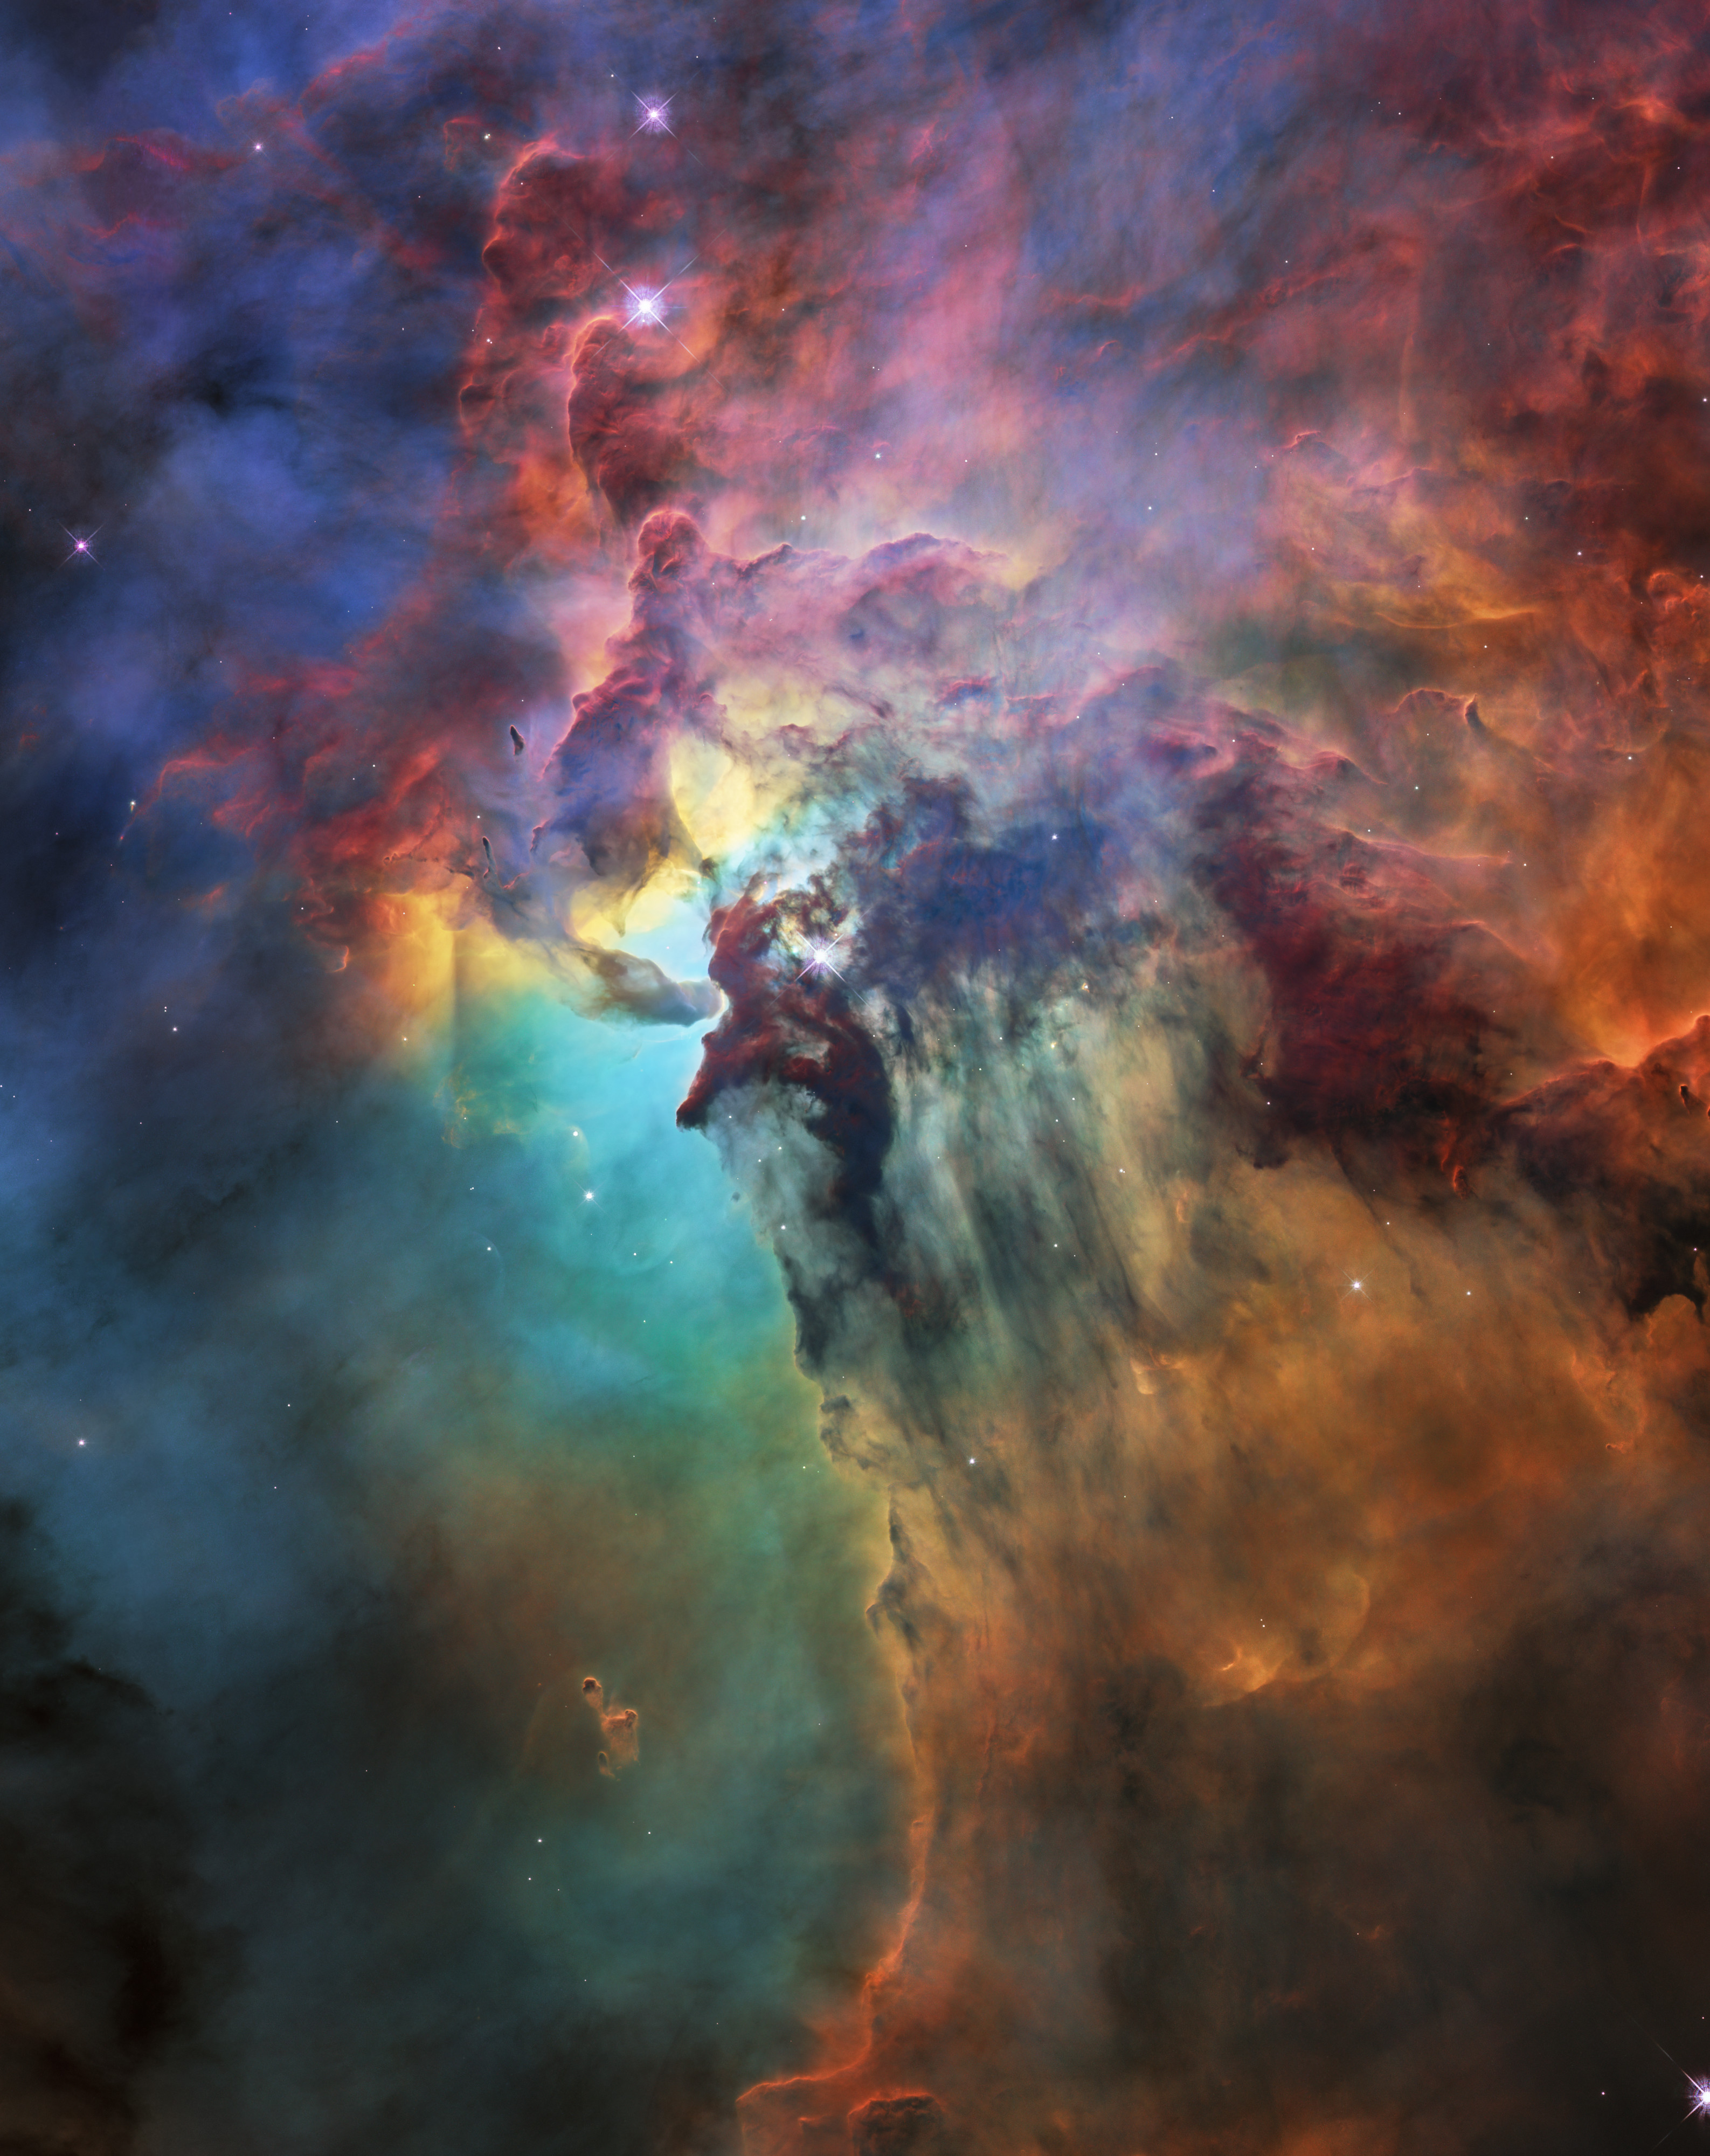
\includegraphics[scale=0.20]{test2}}} % Image background

% --- INIZIO FASCIA SEMI-TRASPARENTE ---
\begin{tikzpicture}[remember picture, overlay]
    \fill[ocre, opacity=0.9] 
        ([yshift=4.5cm]current page.center |- current page.west) rectangle ([yshift=-4cm]current page.center |- current page.east);
\end{tikzpicture}
% --- FINE FASCIA SEMI-TRASPARENTE ---

\centering
\vspace*{6cm}
\par\normalfont\fontsize{35}{35}\sffamily\selectfont
\textbf{Advanced Machine Learning}\\
{\LARGE La Voglia di Morire}\par % Book title
\vspace*{0.5cm}
{\Huge Vincenzo Salvatore}\par % Author name
\vspace*{0.25cm}
{\Huge Raffaele Mercurio}\par % Author name
\endgroup

%----------------------------------------------------------------------------------------
%	COPYRIGHT PAGE
%----------------------------------------------------------------------------------------

\newpage
~\vfill
\thispagestyle{empty}

%\noindent Copyright \copyright\ 2014 Andrea Hidalgo\\ % Copyright notice

\noindent \textsc{Corso di Advanced Machine Learning, Università La Sapienza}\\

%----------------------------------------------------------------------------------------
%	TABLE OF CONTENTS
%----------------------------------------------------------------------------------------

\chapterimage{Pictures/Chapters/Chap1.jpg} % Placeholder image

\pagestyle{empty} % No headers

\tableofcontents % Print the table of contents itself

%\cleardoublepage % Forces the first chapter to start on an odd page so it's on the right

\pagestyle{fancy} % Print headers again

%----------------------------------------------------------------------------------------
%	MOC
%----------------------------------------------------------------------------------------
% ATTENZIONE: Nei file secondari NON devi inserire \begin{document} o \end{document}.
% Inizia subito a scrivere il contenuto!
\newpage

\chapterimage{Pictures/Indice.png}
\chapter{Recap on Machine Learning and Computer Vision}

\section{Introduction to the Core Concepts}

The contents of this chapter are largely based on the introductory slides of the course~\cite{galasso2025recap}.

\begin{keywordbox}
    \begin{itemize}[nosep, leftmargin=*]
    \item According to Arthur Samuel (1959), \textbf{Machine Learning} is the field of study that gives computers the ability to learn without being explicitly programmed. 

    \item Tom Mitchell (1998) defined the well-posed learning problem: a computer program is said to learn from experience $E$ with respect to some task $T$ and some performance measure $P$, if its performance on $T$, as measured by $P$, improves with experience $E$.
    \end{itemize}
\end{keywordbox}

Machine learning is heavily applied in \textbf{Computer Vision}, which can be viewed from three main perspectives: as a science (exploring the computational model of human perception), as engineering (building systems that perceive the world), and through its applications.

\begin{examplebox}
Some typical \textbf{Computer Vision Applications} include:
\begin{itemize}[nosep, leftmargin=*]
    \item \textbf{Medical imaging}: Supporting medical diagnosis and visualization.
    \item \textbf{Surveillance}: Tracking people in airports or train stations.
    \item \textbf{Autonomous driving}: Lane-keeping and pre-crash intervention.
\end{itemize}
\end{examplebox}

\section{Image Classification}

A core task in computer vision is \textbf{Image Classification}: assuming a given set of discrete labels (e.g., \{dog, cat, truck, plane\}), the goal is to map an input digital image to one of these labels.

\begin{figure}[htbp]
    \centering
    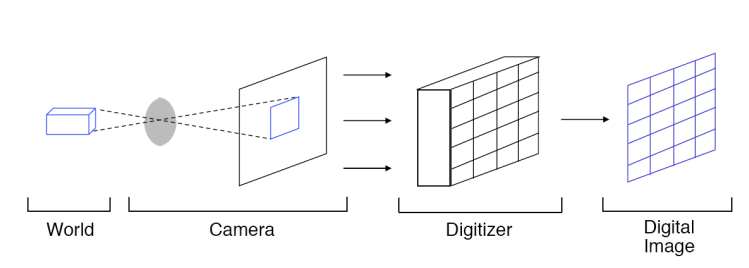
\includegraphics[width=0.7\textwidth]{Pictures/pinhole.png}
    \caption{Illustration of the (pinhole) camera imaging process.}\label{fig:pinhole}
\end{figure}

\begin{Notebox}
\textbf{The Imaging Process:} An image is typically formed via a (pinhole) camera model and then passed through a digitizer to obtain a digital image, which the computer interprets as a large multi-dimensional array of numbers.
\end{Notebox}

\section{Parametric Models and Gradient-Based Optimization}

The majority of machine learning models can be seen as \textbf{Parametric Models}. A parametric model takes an input $x$ and uses a set of parameters (or weights) $W$ and biases $b$ to produce an output prediction $z$:
\[ z = f(x,W) = Wx + b \]

While the exact nature of the prediction depends on the task, what unifies these models is the \textbf{Optimization Process}. We define a Loss function $L$ that measures the error of our predictions, and we iteratively adjust the weights using \textbf{Gradient Descent}:
\[ W^{t+1} = W^t - \alpha \nabla_W L \]
where $\alpha$ is the learning rate.

By simply changing the \textit{activation function} applied to the linear score $z$ and the corresponding \textit{loss function}, we obtain different classical models: Linear Regression, Logistic Regression, and the Softmax Classifier.

\subsection{Linear Regression (\texorpdfstring{$f: \mathbb{R}^D \to \mathbb{R}$}{R -> R})}
Linear Regression is used when the target variable is continuous. We use the identity activation function (i.e., no activation), so the predicted output $\hat{y}$ is exactly the linear score:
\[ \hat{y} = z = Wx + b \]
We optimize this model by minimizing the \textbf{Mean Squared Error (MSE)} loss:
\[ L = \frac{1}{N} \sum_{i=1}^N {(y_i - \hat{y}_i)}^2 \]

\subsection{Logistic Regression (\texorpdfstring{$f: \mathbb{R}^D \to [0, 1]$}{R -> [0, 1]})}
Logistic Regression is used for binary classification. We map the linear score $z$ to a probability between 0 and 1 using the \textbf{Sigmoid} activation function $\sigma(z)$:
\[ P(Y=1 | X=x) = \sigma(z) = \frac{1}{1 + e^{-z}} \]
The appropriate loss function for this model is the \textbf{Binary Cross-Entropy Loss (BCE)}. For a dataset of $N$ samples, it is defined as:
\[ L = -\frac{1}{N} \sum_{i=1}^N \left[ \underbrace{y_i \log(\sigma(z_i))}_{\text{Active if } y=1} + \underbrace{(1 - y_i) \log(1 - \sigma(z_i))}_{\text{Active if } y=0} \right] \]

\begin{Notebox}
\textbf{Understanding the BCE Formula:} This equation uses a clever mathematical trick to combine two mutually exclusive cases into a single line:
\begin{itemize}[nosep, leftmargin=*]
    \item When the true class is \textbf{$y_i = 1$}, the second term $(1 - 1) = 0$ disappears, and the loss evaluates only $-\log(\sigma(z_i))$, penalizing the model if it predicts a low probability.
    \item When the true class is \textbf{$y_i = 0$}, the first term $0$ disappears, and the loss evaluates only $-\log(1 - \sigma(z_i))$, penalizing the model if it predicts a high probability for class 1.
\end{itemize}
\end{Notebox}

\begin{figure}[htbp]
    \centering
    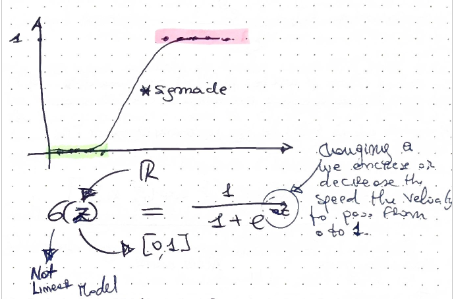
\includegraphics[width=0.7\textwidth]{Pictures/logistic.png}
    \caption{Illustration of the Sigmoid function in Logistic Regression.}\label{fig:logisticregresssion}
\end{figure}

\subsection{Softmax Classifier (\texorpdfstring{$f: \mathbb{R}^D \to \{0, \dots, K\}$}{R -> \{0, \dots, K\}})}
The Softmax Classifier generalizes Logistic Regression to multiple, mutually exclusive classes. It maps the raw scores $z$ into a valid probability distribution over the classes using the \textbf{Softmax function}:
\[ P(Y = k | X = x_i) = \frac{e^{z_k}}{\sum_j e^{z_j}} \]

\begin{Notebox}
\textbf{Why Softmax?} We want to interpret raw classifier scores as \textit{probabilities}. The Softmax function transforms scores such that they are strictly positive and sum to 1.
\end{Notebox}

\begin{examplebox}
For an input image of size $32 \times 32 \times 3$ (e.g., CIFAR-10), the flattened array $x$ has $3072$ numbers. If we are classifying into 10 categories, the weight matrix $W$ will have dimensions $10 \times 3072$, producing a $10 \times 1$ vector of raw class scores before the Softmax is applied.
\end{examplebox}

We then optimize the model using the \textbf{Categorical Cross-Entropy Loss}, often referred to as the Negative Log-Likelihood (NLL). Over the entire dataset of $N$ samples, expanding the Softmax probability formula, the loss becomes:
\[ NLL(W, X) = -\sum_{i=1}^N \left[ \underbrace{W_{y_i}^T x_i}_{\text{Punteggio della classe giusta}} - \underbrace{\log \left( \sum_{k=1}^K \exp(W_k^T x_i) \right)}_{\text{Somma dei punteggi delle altre classi}} \right] \]

\begin{figure}[htbp]
    \centering
    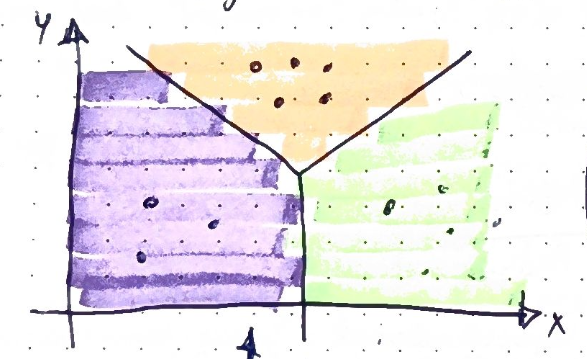
\includegraphics[width=0.7\textwidth]{Pictures/softmax.png}
    \caption{Illustration of the Sigmoid function in Logistic Regression.}\label{fig:Softmax}
\end{figure}

\begin{Notebox}
\textbf{Understanding the Softmax NLL Formula:} 
By looking at the expanded formula, we see that the optimizer tries to maximize the linear score $W_{y_i}^T x_i$ of the \textit{correct class} $y_i$, while simultaneously pushing down the log-sum of the scores of \textit{all available classes}. This creates a competitive environment where increasing the score of the correct class implicitly decreases the relative probability of the others.
\end{Notebox}

\section{Advanced Optimization and Regularization}

\subsection{Regularization}
The primary goal of Regularization is to prevent the model from becoming too complex and overfitting the training data (i.e., we use it to combat \textbf{High Variance}). We achieve this by adding a penalty term $R(W)$, based only on the model's parameters, directly to the Data Loss. 

The new Total Loss becomes:
\[ L_{total}(W, X) = \underbrace{L(W, X)}_{\text{Data Loss}} + \underbrace{\lambda R(W)}_{\text{Regularization Term}} \]

\begin{Notebox}
\textbf{When and how is it applied?}\\
Regularization is applied \textit{during training}. By redefining the Total Loss, we also change its gradient. When we apply Gradient Descent, the algorithm must now minimize both the data error AND the complexity of the weights. For example, the gradient of an L2 penalty $\lambda W^2$ is $2\lambda W$, meaning Gradient Descent will actively shrink the weights at every step (Weight Decay).
\end{Notebox}

The hyperparameter $\lambda$ acts as the ``manipulator'' of complexity:
\begin{itemize}[nosep, leftmargin=*]
    \item $\lambda = 0$: We ignore complexity. The model relies entirely on Data Loss (Risk of \textbf{Overfitting}).
    \item $\lambda \to \infty$: The model becomes ``lazy''. The penalty is so high that Gradient Descent brings all weights to zero (Risk of \textbf{Underfitting}).
\end{itemize}

The two most classic mathematical formulations are:
\begin{itemize}[nosep, leftmargin=*]
    \item \textbf{L2 Regularization (Ridge):} $R(W) = \sum W^2$. It punishes larger weights more severely, forcing the network to distribute the ``weight'' across all features rather than relying heavily on just a few. It shrinks weights but rarely brings them exactly to zero.
    \item \textbf{L1 Regularization (Lasso):} $R(W) = \sum |W|$. It punishes weights constantly. This has the mathematical effect of bringing less important weights exactly to zero, acting as an automatic \textit{Feature Selection} mechanism.
\end{itemize}

\textit{Note: In deep neural networks, we also use architectural regularizers like Dropout and Batch Normalization.}

\subsection{Stochastic Gradient Descent (SGD)}
From a theoretical standpoint, our objective is to minimize the total loss over the entire dataset, which includes both the data loss and the regularization term:
\[ L(W) = \frac{1}{N} \sum_{i=1}^N L_i(x_i, y_i, W) + \lambda R(W) \]
To update the weights, we need the exact gradient of this total loss:
\[ \nabla_W L(W) = \frac{1}{N} \sum_{i=1}^N \nabla_W L_i(x_i, y_i, W) + \lambda \nabla_W R(W) \]

Computing this true gradient (the \textbf{Full Batch} gradient) requires evaluating the sum over all $N$ samples in the dataset at every single step. When $N$ is in the millions, this becomes computationally unfeasible.

\begin{keywordbox}
\textbf{Stochastic Gradient Descent (SGD):} Instead of the full sum, SGD approximates the true gradient by computing the sum over a small \textbf{minibatch} of examples (commonly 32, 64, or 128). This introduces noise but allows for much faster and frequent parameter updates.
\end{keywordbox}

\section{Backpropagation and Neural Networks}

\subsection{Backpropagation}
To update weights, we compute gradients via \textbf{Backpropagation}, which applies the chain rule from the output back to the inputs (backward pass).

\begin{examplebox}
\textbf{Patterns in gradient flow:}
\begin{itemize}[nosep, leftmargin=*]
    \item \textbf{Add gate}: Acts as a gradient distributor.
    \item \textbf{Max gate}: Acts as a gradient router.
    \item \textbf{Mul gate}: Acts as a ``swap multiplier''.
    \item \textbf{Copy gate}: Acts as a gradient adder.
\end{itemize}
\end{examplebox}

\begin{Notebox}
\textbf{Backprop with Matrices:} When inputs and weights are vectors or matrices, local gradients become \textit{Jacobian matrices}. However, Jacobians are often sparse. Instead of explicitly forming them, we use implicit multiplication. A very useful trick to remember: the downstream gradient $dL/dx$ \textbf{always has the same shape} as $x$!
\end{Notebox}

\subsection{Deeper Neural Networks}
By stacking multiple layers and applying non-linear activation functions, we create multi-layer Neural Networks (e.g., $f = W_2 \max(0, W_1 x)$).

\subsection{The Role of Activation Functions}

An \textbf{activation function} is a mathematical ``gate'' applied to the output of a layer ($z = Wx+b$) before passing it to the next layer. Its primary role is to introduce \textbf{non-linearity} into the network. 

\begin{Notebox}
\textbf{Why do we need Non-Linearity?} If we only stacked linear layers without activation functions, the entire deep network would mathematically collapse into a single linear transformation. For example, a 2-layer linear network $f = W_2(W_1 x)$ can be rewritten as $f = W'x$ where $W' = W_2 W_1$. Non-linear activations allow the network to learn and approximate highly complex, non-linear boundaries.
\end{Notebox}

Some of the most common activation functions include:
\begin{itemize}[nosep, leftmargin=*]
    \item \textbf{Sigmoid}: $\sigma(x) = \frac{1}{1 + e^{-x}}$. It squashes numbers to the range $[0, 1]$. Historically popular, but suffers from the \textit{vanishing gradient} problem.
    \item \textbf{tanh}: Squashes numbers to the range $[-1, 1]$. Like sigmoid, its gradients vanish for very large or very small inputs.
    \item \textbf{ReLU (Rectified Linear Unit)}: $f(x) = \max(0, x)$. It is the most widely used default choice because it is computationally efficient and greatly mitigates the vanishing gradient problem.
    \item \textbf{Leaky ReLU} and \textbf{ELU}: Variations of ReLU designed to allow a small, non-zero gradient when $x < 0$ to prevent ``dead neurons''.
\end{itemize}

\input{Chapters/Chapter2.tex}
\input{Chapters/Chapter3.tex}
\input{Chapters/Chapter4.tex}
\input{Chapters/Chapter5.tex}
\input{Chapters/Chapter6.tex}


% --- INIZIO TRUCCO PER LA BIBLIOGRAFIA SENZA IMMAGINE ---
\makeatletter
\let\oldmakeschapterhead\@makeschapterhead % Salviamo il design originale con l'immagine
\renewcommand{\@makeschapterhead}[1]{% Sovrascriviamo il design temporaneamente
  \vspace*{50pt}
  {\noindent\huge\sffamily\bfseries\textcolor{black}{#1}\par} % Stampiamo solo il testo del titolo
  \vspace*{40pt}
}
\makeatother

\printbibliography
\end{document}

